Múltiples \textit{upsets} ocurren cuando varios \textit{bit-flips} se alteran por una sola partícula. Una cantidad de \textit{upsets} en una palabra de la memoria se llama MBUs como se muestra en la figura ~\ref{MBU}, cuando hay varios \textit{upsets} en diferentes palabras de la memoria es referenciado como MCUs como se muestra en la figura ~\ref{MCU}.

Los circuitos integrados tienden a incrementar la sensibilidad a múltiples eventos tipo \textit{upsets} a causa de que las brechas entre los transistores se fabrican cada vez en más pequeñas. Esto permite que se depositen cargas de iones y protones, siendo estas recolectadas por los nodos del circuito causando efectos tipo SEUs en diferentes células de memoria.

\begin{figure}[H]
	\centering
	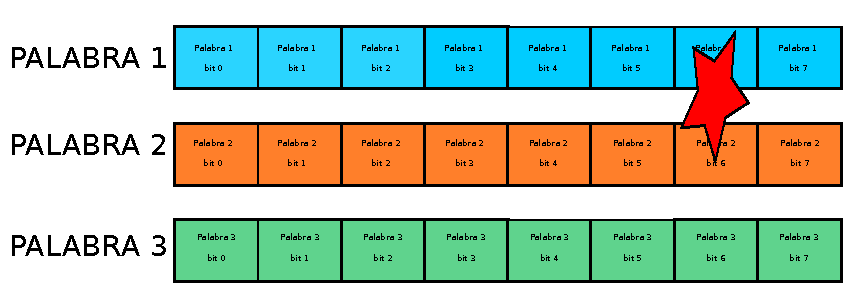
\includegraphics[width=0.6 \textwidth]{img/MCU.pdf}
	\caption{Dos \textit{upsets} en diferentes palabras provocado por una sola partícula (MCU).}
	\label{MCU}
\end{figure}

\begin{figure}[H]
	\centering
	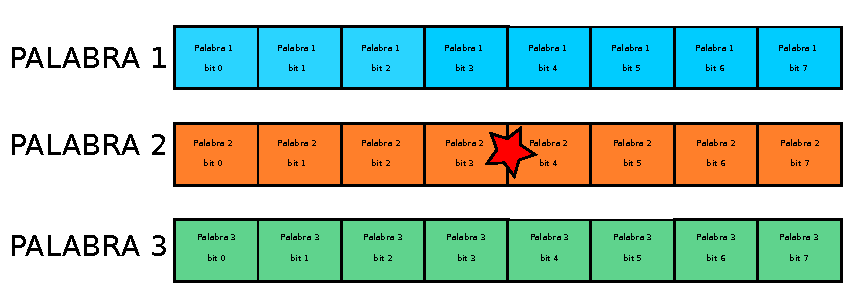
\includegraphics[width=0.6 \textwidth]{img/MBU.pdf}
	\caption{Dos \textit{upsets} en la misma palabra provocada por la misma partícula (MBU).}
	\label{MBU}
\end{figure}